\documentclass[11pt]{article}
\usepackage[margin=1in]{geometry}
\usepackage{booktabs}
\usepackage{amsmath}
\usepackage{threeparttable}
\usepackage{caption}
\usepackage{pgfplots}
\pgfplotsset{compat=1.17}
\usepackage[authoryear,round]{natbib}
\usepackage{setspace}
\setstretch{1.25}
\captionsetup{font=small,labelfont=bf}

\title{Seeing the Supply Base: Mandatory Supplier Disclosure and the Breadth of Reported Supply Networks\\[0.6em]
\large\textbf{SYNTHETIC TEST PAPER, NOT REAL RESEARCH}}
\author{Ilse Varnholt\\University of Castrelle \and Tomas Oyelaran-Brekke\\Maravel School of Management}
\date{Working paper}

\begin{document}
\maketitle

\begin{abstract}
\noindent Firms know less about their supply networks than their contracts suggest, and much of what they know stays inside the procurement function. We study whether a legal mandate to disclose suppliers changes how many suppliers firms report. Between 2011 and 2019 the 42 regions of the Republic of Maravel adopted the Supply Chain Disclosure Act in five cohorts. Using a panel of 3,150 manufacturing firms observed from 2005 to 2019, we find that adoption of the law increased the number of suppliers a firm reports by 2.84 (standard error 1.12), about 7 percent of the pre-period mean. The law also raised the number of on-site supplier audits firms conduct. The findings suggest that disclosure mandates widen the part of the supply base that firms are willing to make visible, and that visibility is followed by monitoring.
\end{abstract}

\section{Introduction}

Supply networks have become longer and harder to see. A manufacturer that buys from forty direct suppliers may depend on several hundred firms two or three tiers away, and most managers cannot name them. Research on supply chain transparency has asked whether firms that disclose more about their suppliers are rewarded by customers and investors, and whether disclosure changes the way firms govern their suppliers. Most of that work studies voluntary disclosure, which makes it hard to separate the effect of disclosure from the kind of firm that chooses to disclose.

Mandatory disclosure laws offer a way around this problem. When a government requires every firm in a jurisdiction to publish a list of its suppliers, the decision to disclose no longer reflects the firm's own choice. What remains open is how firms respond. A firm could meet the mandate with the shortest list the law permits. It could also use the mandate as an occasion to map its supply base and report suppliers it had never recorded in one place. Which response dominates matters for regulators, who hope that disclosure will improve oversight of distant suppliers, and for managers, who must decide how much of the supply base to expose.

We study this question in the Republic of Maravel, where the Supply Chain Disclosure Act (SCDA) required firms with more than fifty employees to publish an annual register of their direct and second-tier suppliers. Maravel's 42 regions adopted the law at different times: six regions in 2011, eight in 2013, nine in 2015, seven in 2017, and twelve in 2019. This staggered adoption lets us compare firms in regions that had adopted the law with firms in regions that had not yet done so, before and after each adoption.

Our data come from the Maravel Registry of Corporate Disclosures, which collects the annual filings of all incorporated manufacturers, and from the regional labor inspectorates, which record firm headcount. The panel covers 3,150 firms from 2005 to 2019. We find that the SCDA raised the number of suppliers a firm reports by 2.84, about 7 percent of the pre-period mean of 38.6. The effect grows over the first years after adoption, which fits the idea that firms learn about their supply base as they build the systems the law requires. We also find that the law raised the number of on-site audits firms conduct of their suppliers.

The paper makes two contributions. First, it provides evidence that disclosure mandates change what firms know and report about their supply networks, not only what they say about them. Second, it links disclosure to monitoring, showing that the act of listing suppliers is followed by closer oversight.

\section{Setting: The Supply Chain Disclosure Act}

Maravel is a mid-sized manufacturing economy with a federal structure. Its 42 regions set most commercial regulation, and regional assemblies can adopt model laws drafted by the national Commerce Council. The Council drafted the SCDA in 2008 after a series of labor scandals at second-tier textile suppliers. The model law requires every firm with more than fifty employees to file, each year, a register listing each direct supplier and each second-tier supplier the firm is aware of, with the supplier's name, location, and the product category supplied. Registers are filed with the regional commerce office and are public.

Regional assemblies adopted the model law at different times, for reasons that the regional press attributes mostly to legislative calendars and to the order in which regional commerce offices built the filing systems. Each regional assembly announced its adoption two years before the law took effect, giving firms time to build the internal systems needed to compile the register. The effective year is the first fiscal year for which a register must be filed. Table~\ref{tab:cohorts} lists the announcement and effective years for each adoption cohort.

\begin{table}[ht]
\centering
\begin{threeparttable}
\caption{Adoption cohorts of the Supply Chain Disclosure Act}
\label{tab:cohorts}
\small
\begin{tabular}{lccccc}
\toprule
Cohort & Announced & Effective & Regions & Firms & Firm-years \\
\midrule
2011 & 2009 & 2011 & 6 & 480 & 7,200 \\
2013 & 2011 & 2013 & 8 & 620 & 9,300 \\
2015 & 2013 & 2015 & 9 & 710 & 10,650 \\
2017 & 2015 & 2017 & 7 & 540 & 8,100 \\
2019 & 2017 & 2019 & 12 & 800 & 12,000 \\
\midrule
Total & & & 42 & 3,150 & 47,250 \\
\bottomrule
\end{tabular}
\begin{tablenotes}\footnotesize
\item Notes: Firms are manufacturers with more than fifty employees in every year from 2005 to 2019. The panel is balanced, so each firm contributes fifteen firm-years.
\end{tablenotes}
\end{threeparttable}
\end{table}

No region repealed, suspended, or amended the law during the sample period, and no firm that became subject to the law was later released from it. Treatment is therefore absorbing: once a region's law takes effect, every firm in that region remains treated through 2019. Firms could not escape the law by moving their registered office, because the SCDA applies to the region in which a firm's main production site is located, and no firm in our panel moved its main site across a regional border.

\section{Theory and Hypotheses}

A supplier register asks a firm to write down something it may never have assembled. Direct suppliers appear in the accounts payable ledger, but second-tier suppliers are known only through conversations with direct suppliers, audit reports, and product specifications. Before the mandate, a firm has little reason to pull this knowledge together. After the mandate, the firm must file a list, and the cost of an omission discovered by a journalist or a regulator is borne by the firm.

Two responses are possible. A minimal response lists only direct suppliers and the few second-tier suppliers that are already documented. An expansive response treats the mandate as a reason to map the supply base, asking direct suppliers to name their own suppliers and recording them in one place. We expect the expansive response to dominate for two reasons. First, the public register makes omissions visible to competitors and journalists, who can compare the lists of firms that share suppliers. Second, the systems firms build to comply lower the cost of adding a supplier to the list once the first register is filed.

\textit{Hypothesis 1 (H1): Adoption of the Supply Chain Disclosure Act increases the number of suppliers a firm reports.}

Once a firm has listed its suppliers, it becomes answerable for them. A supplier that appears on a public register and is later found to use forced labor is a reputational liability that the firm cannot plausibly deny knowing about. We therefore expect disclosure to be followed by monitoring.

\textit{Hypothesis 2 (H2): Adoption of the Supply Chain Disclosure Act increases the number of on-site audits a firm conducts of its suppliers.}

\section{Data and Methods}

\subsection{Sample and measures}

We draw firm filings from the Maravel Registry of Corporate Disclosures (MRCD), which holds the annual reports of all incorporated manufacturers from 2003 onward. Before the SCDA, firms reported suppliers in an optional schedule of the annual report, which the MRCD digitizes; after the SCDA, the regional registers replace that schedule. The MRCD harmonizes the two sources so that the count of reported suppliers is measured in the same way before and after adoption. Our sample is the 3,150 manufacturers with more than fifty employees in every year from 2005 to 2019, giving a balanced panel of 47,250 firm-years.

The outcome for H1 is the number of distinct suppliers, direct and second-tier, that the firm reports in a year. The outcome for H2 is the number of on-site supplier audits the firm reports conducting in the year, which firms have disclosed in the MRCD's governance schedule since 2004. Headcount comes from the regional labor inspectorates and is the number of employees on the payroll at the end of the fiscal year. Regional GDP growth comes from Maravel's statistical office. Table~\ref{tab:desc} reports descriptive statistics.

\begin{table}[ht]
\centering
\begin{threeparttable}
\caption{Descriptive statistics}
\label{tab:desc}
\small
\begin{tabular}{lccccc}
\toprule
Variable & Mean & SD & Min & Max & N \\
\midrule
Suppliers reported & 38.6 & 21.4 & 3 & 214 & 47,250 \\
Supplier audits & 4.2 & 3.1 & 0 & 31 & 47,250 \\
Headcount (employees) & 412 & 588 & 51 & 9,840 & 47,250 \\
Log headcount & 5.12 & 1.34 & 3.93 & 9.19 & 47,250 \\
Regional GDP growth (\%) & 2.3 & 1.9 & $-$4.8 & 7.6 & 47,250 \\
\bottomrule
\end{tabular}
\begin{tablenotes}\footnotesize
\item Notes: Firm-year observations, 2005 to 2019. Pre-period mean of suppliers reported (firm-years before each firm's region adopted the law): 38.6. No variable has missing values in the balanced panel.
\end{tablenotes}
\end{threeparttable}
\end{table}

\subsection{Empirical strategy}

We estimate the effect of the SCDA with a two-way fixed effects difference-in-differences model. Treated firms are those in the thirty regions that adopted the law in 2011, 2013, 2015, or 2017. The twelve never-treated regions serve as the control group throughout. Our main specification is
\begin{equation}
Y_{irt} = \beta \, \text{SCDA}_{rt} + \gamma \log(\text{Headcount}_{irt}) + \delta \, \text{GDPGrowth}_{rt} + \alpha_i + \tau_t + \varepsilon_{irt},
\end{equation}
where $Y_{irt}$ is the outcome for firm $i$ in region $r$ in year $t$, $\text{SCDA}_{rt}$ equals one from the year the law took effect in region $r$ onward, $\alpha_i$ are firm fixed effects, and $\tau_t$ are year fixed effects. We control for the firm's log headcount in the current year, because larger firms have more suppliers, and for regional GDP growth, because regional demand shocks could shift purchasing. Standard errors are clustered by region, the level at which the law was assigned, which gives 42 clusters.

To trace the timing of the effect, we also estimate an event-study version of the model that replaces $\text{SCDA}_{rt}$ with indicators for each year relative to adoption, with the year before adoption as the omitted reference year. The identifying assumption is that, absent the law, the number of suppliers reported by firms in adopting regions would have evolved in parallel with that of firms in the control regions.

\section{Results}

\subsection{Main estimates}

Table~\ref{tab:main} reports the estimates for H1. Column 1 includes only firm and year fixed effects and gives an estimate of 3.05 (standard error 1.20). Column 2 adds log headcount and regional GDP growth and is our preferred specification. Adoption of the SCDA increased the number of reported suppliers by 2.84 (standard error 1.12, $p < 0.05$), or 7.4 percent of the pre-period mean of 38.6. Column 3 uses the log of one plus the supplier count as the outcome and gives 0.071 (standard error 0.029), a proportional effect close to the one implied by column 2. We use the count in levels in the main analysis because the count is never zero in our sample and a supplier added to the register has the same meaning for a small and a large firm. H1 is supported.

\begin{table}[ht]
\centering
\begin{threeparttable}
\caption{Effect of the SCDA on the number of suppliers reported}
\label{tab:main}
\small
\begin{tabular}{lccc}
\toprule
 & (1) & (2) & (3) \\
 & Suppliers & Suppliers & Log(1 + suppliers) \\
\midrule
SCDA in effect & 3.05** & 2.84** & 0.071** \\
 & (1.20) & (1.12) & (0.029) \\
Log headcount & & 4.36*** & 0.108*** \\
 & & (1.02) & (0.024) \\
Regional GDP growth & & 0.21 & 0.004 \\
 & & (0.14) & (0.003) \\
\midrule
Firm fixed effects & Yes & Yes & Yes \\
Year fixed effects & Yes & Yes & Yes \\
Firm-years & 47,250 & 47,250 & 47,250 \\
Firms & 3,150 & 3,150 & 3,150 \\
Regions (clusters) & 42 & 42 & 42 \\
Within $R^2$ & 0.021 & 0.064 & 0.059 \\
\bottomrule
\end{tabular}
\begin{tablenotes}\footnotesize
\item Notes: Two-way fixed effects estimates. Standard errors clustered by region in parentheses. *** $p<0.01$, ** $p<0.05$, * $p<0.10$.
\end{tablenotes}
\end{threeparttable}
\end{table}

\subsection{Event-study estimates}

Table~\ref{tab:es} and Figure~\ref{fig:es} report the event-study estimates. The five leads are small and none is individually distinguishable from zero. The joint test of the five leads ($p = 0.31$) confirms the identifying assumption. After adoption, the estimates rise steadily: the effect is 1.02 in the year the law takes effect, crosses conventional significance in the third year, and reaches 4.62 six years after adoption. The rising pattern is consistent with firms learning about their supply base over time and adding second-tier suppliers to the register as their mapping systems mature.

\begin{table}[ht]
\centering
\begin{threeparttable}
\caption{Event-study estimates: suppliers reported}
\label{tab:es}
\small
\begin{tabular}{lcc|lcc}
\toprule
Event time & Estimate & SE & Event time & Estimate & SE \\
\midrule
$-6$ & 0.88 & (1.94) & $0$ & 1.02 & (1.21) \\
$-5$ & $-$0.61 & (1.83) & $+1$ & 2.10 & (1.30) \\
$-4$ & 1.12 & (1.71) & $+2$ & 2.95** & (1.38) \\
$-3$ & $-$0.47 & (1.72) & $+3$ & 3.60** & (1.52) \\
$-2$ & 0.35 & (1.49) & $+4$ & 3.88** & (1.70) \\
$-1$ & 0 & (ref.) & $+5$ & 4.41** & (1.95) \\
 & & & $+6$ & 4.62** & (2.10) \\
\midrule
\multicolumn{6}{l}{Joint test of leads $-6$ to $-2$: $F(5, 41) = 1.22$, $p = 0.31$} \\
\multicolumn{6}{l}{Firm-years 47,250; firms 3,150; regions (clusters) 42} \\
\bottomrule
\end{tabular}
\begin{tablenotes}\footnotesize
\item Notes: Two-way fixed effects event-study regression with firm and year fixed effects, log headcount, and regional GDP growth. Standard errors clustered by region in parentheses. *** $p<0.01$, ** $p<0.05$, * $p<0.10$.
\end{tablenotes}
\end{threeparttable}
\end{table}

\begin{figure}[ht]
\centering
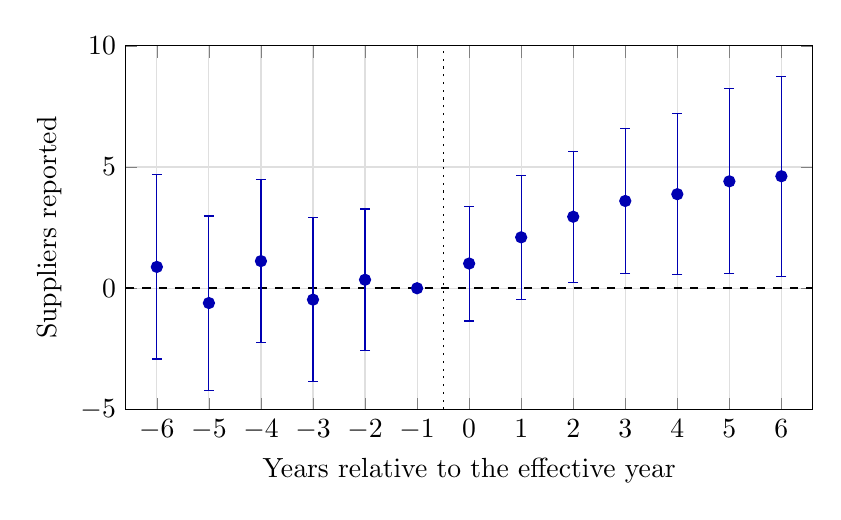
\begin{tikzpicture}
\begin{axis}[
  width=0.85\textwidth, height=6.2cm,
  xlabel={Years relative to the effective year},
  ylabel={Suppliers reported},
  xmin=-6.6, xmax=6.6, ymin=-5, ymax=10,
  xtick={-6,-5,-4,-3,-2,-1,0,1,2,3,4,5,6},
  grid=major, grid style={gray!25},
  every axis plot/.append style={thick}
]
\addplot[black, dashed, domain=-6.6:6.6, samples=2] {0};
\addplot[black, dotted, thin] coordinates {(-0.5,-5) (-0.5,10)};
\addplot[blue!70!black, only marks, mark=*, mark size=1.8pt,
  error bars/.cd, y dir=both, y explicit]
  coordinates {
  (-6,0.88) +- (0,3.80)
  (-5,-0.61) +- (0,3.59)
  (-4,1.12) +- (0,3.35)
  (-3,-0.47) +- (0,3.37)
  (-2,0.35) +- (0,2.92)
  (-1,0) +- (0,0)
  (0,1.02) +- (0,2.37)
  (1,2.10) +- (0,2.55)
  (2,2.95) +- (0,2.70)
  (3,3.60) +- (0,2.98)
  (4,3.88) +- (0,3.33)
  (5,4.41) +- (0,3.82)
  (6,4.62) +- (0,4.12)
  };
\end{axis}
\end{tikzpicture}
\caption{Event-study estimates of the effect of the SCDA on suppliers reported. Coefficients for event times $-6$ to $+6$ relative to the year the law took effect, with 95 percent confidence intervals based on standard errors clustered by region. Event time $-1$ is the omitted reference year. Leads before $-6$ are binned into $-6$ and lags after $+6$ are binned into $+6$. Estimates are from Table~\ref{tab:es}.}
\label{fig:es}
\end{figure}

\subsection{Compliance staffing}

Building a supplier register takes people. Regional commerce offices advised firms to appoint a compliance officer for the register, and industry associations reported that many firms added procurement analysts to trace second-tier suppliers. Table~\ref{tab:staff} shows that the SCDA raised firm headcount. Adoption increased log headcount by 0.041 (standard error 0.016), or about 4.1 percent, in the same two-way fixed effects specification with regional GDP growth as the only control. The law therefore increased firms' headcount, and the increase is concentrated in the first three years after adoption, when firms were building their registers.

\begin{table}[ht]
\centering
\begin{threeparttable}
\caption{Effect of the SCDA on firm headcount}
\label{tab:staff}
\small
\begin{tabular}{lc}
\toprule
 & Log headcount \\
\midrule
SCDA in effect & 0.041** \\
 & (0.016) \\
Regional GDP growth & 0.006** \\
 & (0.003) \\
\midrule
Firm and year fixed effects & Yes \\
Firm-years & 47,250 \\
Regions (clusters) & 42 \\
\bottomrule
\end{tabular}
\begin{tablenotes}\footnotesize
\item Notes: Two-way fixed effects estimates. Standard errors clustered by region in parentheses. *** $p<0.01$, ** $p<0.05$, * $p<0.10$.
\end{tablenotes}
\end{threeparttable}
\end{table}

\subsection{Robustness}

Appendix A reports an estimate from the heterogeneity-robust estimator of \citet{cs2021}, which we compare with our two-way fixed effects estimate. Appendix B reports a synthetic control analysis for Harrowmere, the largest region to adopt the law, which gives a region-level effect of the same sign and similar size as our firm-level estimate.

\section{Supplier Audits}

We test H2 with the estimator of Callaway and Sant'Anna (2021). The number of audits is a small count with a pre-period mean of 3.6, and we want an event study whose leads and lags are not contaminated by effects from other relative periods. Because each law was announced two years before it took effect, firms could begin to respond before the effective year, so we allow two years of anticipation. The base period is therefore $e = -3$, the last year before the announcement, and every lead and lag is measured relative to it (a universal base period). Controls are not-yet-treated regions whose law had not yet been announced in the comparison year, with no covariates. The last cohort's law was announced in 2017, so no unannounced region remains after 2016 and group-time effects are estimated for 2005 to 2016. Within that window we estimate group-time effects for the 2011, 2013, and 2015 cohorts. The 2017 cohort's post-adoption effects are not identified, because by 2017 every remaining region had announced its law; the 2017 and 2019 cohorts serve only as controls in earlier years. We aggregate group-time effects into event-time effects with weights proportional to cohort size and restrict the window to event times $-6$ to $+1$, which keeps it balanced: each of the three cohorts contributes to every event time in that window. Event times $-2$ and $-1$ fall inside the anticipation window and are reported as estimated effects, not as pre-trend tests. Standard errors come from a multiplier bootstrap with 1,000 draws, clustered by region.

Table~\ref{tab:audit} reports the estimates. The three pre-announcement leads ($e = -6$ to $-4$) range from $-0.01$ to $0.02$ and show no drift. In the anticipation years the estimates are 0.06 and 0.14, small and imprecise. The effect is 0.52 audits in the effective year and 0.80 in the following year. The average of the two post-period effects is 0.66 (standard error 0.18), about 18 percent of the pre-period mean.

\begin{table}[ht]
\centering
\begin{threeparttable}
\caption{Effect of the SCDA on supplier audits: Callaway and Sant'Anna event study}
\label{tab:audit}
\small
\begin{tabular}{lcc}
\toprule
Event time & Estimate & SE \\
\midrule
$-6$ & 0.02 & (0.17) \\
$-5$ & $-$0.01 & (0.16) \\
$-4$ & 0.02 & (0.15) \\
$-3$ & 0 & (base) \\
$-2$ (anticipation) & 0.06 & (0.15) \\
$-1$ (anticipation) & 0.14 & (0.16) \\
$0$ & 0.52*** & (0.19) \\
$+1$ & 0.80*** & (0.24) \\
\midrule
Average of $e = 0$ and $e = +1$ & 0.66*** & (0.18) \\
\midrule
\multicolumn{3}{l}{Honest DiD, relative magnitudes (average post effect)} \\
\quad 95\% robust CI at $\bar{M} = 1$ & \multicolumn{2}{c}{[0.20, 1.12]} \\
\quad Breakdown value $\bar{M}$ & \multicolumn{2}{c}{2.9} \\
\midrule
Firm-years & \multicolumn{2}{c}{37,800} \\
Regions (clusters) & \multicolumn{2}{c}{42} \\
\bottomrule
\end{tabular}
\begin{tablenotes}\footnotesize
\item Notes: Callaway and Sant'Anna (2021) estimates for the 2011, 2013, and 2015 cohorts with two years of anticipation, a universal base period ($e = -3$), controls limited to regions whose law had not yet been announced, no covariates, and cohort-size aggregation weights. Firm-years cover 2005 to 2016 (3,150 firms $\times$ 12 years). Standard errors from a multiplier bootstrap (1,000 draws) clustered by region. *** $p<0.01$, ** $p<0.05$, * $p<0.10$.
\end{tablenotes}
\end{threeparttable}
\end{table}

A flat set of leads does not prove parallel trends, because a pre-trend test can have little power against violations large enough to matter \citep{roth2022}. We therefore follow \citet{rr2023} and bound the post-period violation of parallel trends by a multiple $\bar{M}$ of the largest change between consecutive pre-period coefficients, which in Table~\ref{tab:audit} is 0.03 (between $e = -6$ and $e = -5$, and again between $e = -5$ and $e = -4$). Because the base period is $e = -3$, the effects at $e = 0$ and $e = +1$ lie three and four periods after it, so the largest violation of the average post-period effect allowed at a given $\bar{M}$ is $3.5 \times 0.03 \times \bar{M} = 0.105\bar{M}$. The average post-period effect remains positive for any $\bar{M}$ up to 2.9, the breakdown value; at $\bar{M} = 1$ the robust 95 percent confidence interval is [0.20, 1.12]. We regard $\bar{M} = 1$ as the relevant benchmark. A violation of that size would require audit demand in adopting regions to shift, in the year of adoption, by as much as the largest year-to-year swing observed over the six pre-adoption years, a period that included the 2008 textile scandals that prompted the model law. We see no event in the adoption years of comparable size, so we conclude that the SCDA raised supplier audits under violations of parallel trends as large as the largest pre-period swing and up to 2.9 times that size. H2 is supported.

\section{Discussion}

Mandatory disclosure is often criticized as a paperwork exercise: firms comply at the lowest cost, and the information disclosed changes little. Our results suggest a different reading for supply chains. When the SCDA required firms to list their suppliers, firms listed more of them than before, and the lists grew as the firms' systems matured. The law also raised supplier audits, which suggests that making the supply base visible makes firms answerable for it.

The findings have implications for managers. A disclosure mandate imposes a fixed cost of building a register, reflected in the compliance staffing we observe. Once that cost is paid, the marginal cost of mapping more of the supply base is low, and firms appear to use the systems they built. Managers facing a similar mandate may do better to treat it as an occasion to map the supply base than as a filing obligation.

The study has limits. We observe what firms report, not the true size of their supply networks, so we cannot say whether firms discovered new suppliers or disclosed suppliers they already knew. Maravel's regions differ from one another less than countries do, which helps comparison but limits how far the results travel. Future work could link the registers across firms to study how disclosure spreads along a supply chain.

\section{Conclusion}

Staggered adoption of the Supply Chain Disclosure Act across Maravel's 42 regions increased the number of suppliers firms report by 2.84, about 7 percent, and increased supplier audits. Disclosure mandates appear to widen the visible supply base and to be followed by closer monitoring of it.

\begin{thebibliography}{99}
\setlength{\itemsep}{2pt}
\small

\bibitem[Abadie et al.(2010)]{adh2010} Abadie, A., Diamond, A., and Hainmueller, J. (2010). Synthetic control methods for comparative case studies: estimating the effect of California's tobacco control program. \textit{Journal of the American Statistical Association}, 105(490), 493--505.

\bibitem[Baker et al.(2022)]{blw2022} Baker, A. C., Larcker, D. F., and Wang, C. C. Y. (2022). How much should we trust staggered difference-in-differences estimates? \textit{Journal of Financial Economics}, 144(2), 370--395.

\bibitem[Callaway and Sant'Anna(2021)]{cs2021} Callaway, B., and Sant'Anna, P. H. C. (2021). Difference-in-differences with multiple time periods. \textit{Journal of Econometrics}, 225(2), 200--230.

\bibitem[Goodman-Bacon(2021)]{gb2021} Goodman-Bacon, A. (2021). Difference-in-differences with variation in treatment timing. \textit{Journal of Econometrics}, 225(2), 254--277.

\bibitem[Rambachan and Roth(2023)]{rr2023} Rambachan, A., and Roth, J. (2023). A more credible approach to parallel trends. \textit{Review of Economic Studies}, 90(5), 2555--2591.

\bibitem[Roth(2022)]{roth2022} Roth, J. (2022). Pretest with caution: event-study estimates after testing for parallel trends. \textit{American Economic Review: Insights}, 4(3), 305--322.

\bibitem[Roth et al.(2023)]{rsbp2023} Roth, J., Sant'Anna, P. H. C., Bilinski, A., and Poe, J. (2023). What's trending in difference-in-differences? A synthesis of the recent econometrics literature. \textit{Journal of Econometrics}, 235(2), 2218--2244.

\bibitem[Sun and Abraham(2021)]{sa2021} Sun, L., and Abraham, S. (2021). Estimating dynamic treatment effects in event studies with heterogeneous treatment effects. \textit{Journal of Econometrics}, 225(2), 175--199.

\end{thebibliography}

\clearpage
\appendix
\section*{Appendix A: Heterogeneity-Robust Estimate for Suppliers Reported}
\addcontentsline{toc}{section}{Appendix A}

When adoption is staggered and effects vary across cohorts or over time, a two-way fixed effects coefficient can place weight on comparisons that use already-treated regions as controls \citep{gb2021, sa2021, rsbp2023}. As a check, we estimate the overall effect of the SCDA on suppliers reported with the estimator of \citet{cs2021}.

Because every region adopts the law by 2019, there are no never-treated regions, and we use not-yet-treated regions as controls. Because each law was announced two years before it took effect, we allow two years of anticipation: the universal base period is three years before each cohort's effective year ($e = -3$), the last year before the announcement, and controls are limited to regions whose law had not yet been announced in the comparison year. No unannounced region remains after 2016, so group-time effects are estimated for 2005 to 2016. This identifies post-adoption effects for the 2011, 2013, and 2015 cohorts; the 2017 cohort's effects are not identified, and the 2017 and 2019 cohorts serve only as controls in earlier years. We include no covariates. We first average each cohort's group-time effects over its post-adoption years in the estimation window, then aggregate the three cohort effects into an overall effect with weights proportional to the number of firms in each cohort (480, 620, and 710 firms, 1,810 in total). Standard errors come from a multiplier bootstrap with 1,000 draws, clustered by region.

\begin{table}[ht]
\centering
\begin{threeparttable}
\caption{Callaway and Sant'Anna estimates: suppliers reported}
\label{tab:cs}
\small
\begin{tabular}{lcccc}
\toprule
Cohort & Firms & Weight & ATT & SE \\
\midrule
2011 & 480 & 0.265 & $-$2.61 & (1.84) \\
2013 & 620 & 0.343 & $-$1.37 & (1.52) \\
2015 & 710 & 0.392 & $-$0.24 & (1.41) \\
2017 & 540 & \multicolumn{3}{c}{not identified} \\
\midrule
Overall ATT & 1,810 & 1.000 & $-$1.26 & (1.14) \\
\midrule
\multicolumn{5}{l}{Firm-years 37,800; regions (clusters) 42} \\
\bottomrule
\end{tabular}
\begin{tablenotes}\footnotesize
\item Notes: Callaway and Sant'Anna (2021) estimates with two years of anticipation, a universal base period ($e = -3$), controls limited to regions whose law had not yet been announced, no covariates, and cohort aggregation weights proportional to the number of firms. The overall ATT is the weighted average of the three identified cohort ATTs. Firm-years cover 2005 to 2016 (3,150 firms $\times$ 12 years). Standard errors from a multiplier bootstrap (1,000 draws) clustered by region in parentheses. *** $p<0.01$, ** $p<0.05$, * $p<0.10$.
\end{tablenotes}
\end{threeparttable}
\end{table}

Table~\ref{tab:cs} reports the results. The overall ATT of $-1.26$ (standard error 1.14) is similar to our main two-way fixed effects estimate, and we conclude that our main result is not an artifact of staggered adoption.

\clearpage
\section*{Appendix B: Synthetic Control for Harrowmere}
\addcontentsline{toc}{section}{Appendix B}

As a supporting analysis, we build a synthetic control \citep{adh2010} for Harrowmere, the largest region to adopt the law (148 firms, 2013 cohort). The outcome is the mean number of suppliers reported per firm in the region. The pre-period is 2005 to 2012 (eight years) and the post-period is 2013 to 2016. We end the post-period in 2016 because the donor regions announced their own adoption in 2017.

The donor pool follows a stated rule. Donors must be untreated throughout the analysis window and not yet announced, which leaves the twelve regions of the 2019 cohort. We drop three of these: two whose main ports closed for most of 2014, and one whose largest manufacturer entered receivership in 2012. The remaining nine regions form the donor pool. We keep regions that share Harrowmere's exposure to national demand and exchange-rate shocks. Predictors are the mean supplier count in 2005 to 2007 and in 2008 to 2010, mean log headcount in 2005 to 2010, and the manufacturing share of regional output in 2010, all measured before the law was announced in Harrowmere (2011).

\begin{table}[ht]
\centering
\begin{threeparttable}
\caption{Synthetic control for Harrowmere: predictor balance and donor weights}
\label{tab:sc}
\small
\begin{tabular}{lccc}
\toprule
\multicolumn{4}{l}{\textit{Panel A. Predictor balance}} \\
 & Harrowmere & Synthetic & Donor average \\
\midrule
Suppliers reported, 2005 to 2007 & 36.9 & 37.2 & 33.4 \\
Suppliers reported, 2008 to 2010 & 39.8 & 39.5 & 35.1 \\
Log headcount, 2005 to 2010 & 5.31 & 5.27 & 4.98 \\
Manufacturing share, 2010 (\%) & 31.4 & 30.8 & 27.6 \\
\midrule
\multicolumn{4}{l}{\textit{Panel B. Donor weights}} \\
\multicolumn{3}{l}{Ostwick} & 0.34 \\
\multicolumn{3}{l}{Lindqvar} & 0.27 \\
\multicolumn{3}{l}{Pellmar} & 0.21 \\
\multicolumn{3}{l}{Sorrendale} & 0.18 \\
\multicolumn{3}{l}{Five other donors} & 0.00 \\
\midrule
\multicolumn{4}{l}{\textit{Panel C. Fit and effect}} \\
\multicolumn{3}{l}{Pre-period RMSPE (suppliers), 2005 to 2012} & 0.84 \\
\multicolumn{3}{l}{Gap by year, 2013 / 2014 / 2015 / 2016} & 1.9 / 2.8 / 3.5 / 4.2 \\
\multicolumn{3}{l}{Mean post-period gap, 2013 to 2016} & 3.10 \\
\multicolumn{3}{l}{Post-period RMSPE / pre-period RMSPE} & 3.83 \\
\bottomrule
\end{tabular}
\begin{tablenotes}\footnotesize
\item Notes: Synthetic control with non-negative weights summing to one, fitted on the four predictors listed in Panel A. Nine donor regions. The standard deviation of the region's year-to-year change in mean suppliers reported over 2005 to 2012 is 1.1.
\end{tablenotes}
\end{threeparttable}
\end{table}

Table~\ref{tab:sc} reports the results. The synthetic control tracks Harrowmere closely before 2013, with a pre-period RMSPE of 0.84 suppliers, and Harrowmere lies within the donors' range on every predictor. Four donors receive positive weight. After the law takes effect, Harrowmere's mean supplier count rises above its synthetic control by 1.9 suppliers in 2013 and 4.2 in 2016, for a mean gap of 3.10, several times the region's typical year-to-year change of 1.1. Dropping each positive-weight donor in turn gives mean gaps between 2.71 and 3.46, and replacing the two supplier predictors with the eight annual pre-period outcomes gives 3.24. We report the four-predictor specification because it was fixed before we examined post-period outcomes. Backdating the law to 2009 and fitting on 2005 to 2008 gives a mean placebo gap of 0.21 for 2009 to 2012.

For inference we run in-space placebos, assigning the law to each of the nine donor regions in turn and computing the ratio of post-period to pre-period RMSPE. We keep every placebo. Harrowmere's ratio of 3.83 is the largest of the ten, which gives a permutation p-value of 0.03, significant at 5 percent. We read this as evidence that the gap in Harrowmere is unusual relative to the donor regions, and we do not generalize the size of the effect beyond Harrowmere.

\end{document}
